\documentclass[aps,reprint]{revtex4-1}

\usepackage[english]{babel}
\usepackage{csquotes}
% \usepackage[backend=biber, sortcites]{biblatex}
\usepackage{url}
\usepackage{textcomp}
\usepackage[usenames,dvipsnames,svgnames, table]{xcolor}
\usepackage[font={scriptsize}]{caption}
\usepackage{amsmath} \usepackage{amsthm} \usepackage{amsfonts}
\usepackage{amssymb}
\usepackage{enumerate}
\usepackage{tikz} \usepackage{float}
\usepackage[procnames]{listings}
\usepackage{pstool} \usepackage{pgfplots}
\usepackage{wrapfig} \usepackage{graphicx} \usepackage{epstopdf}
\usepackage{afterpage}
\usepackage{physics}
\usepackage{multirow}
\usepackage{gensymb}
\usepackage{algorithm}
\usepackage{microtype}
\usepackage[noend]{algpseudocode}
\usepackage{xcolor,colortbl}
\usepackage{microtype}
\usepackage{geometry}
\usepackage{hyperref}
\usepackage{graphicx}
\usepackage{caption}
\usepackage{subcaption}
\usepackage{lipsum}
% \usepackage{pythontex}
% \usepackage{authblk}
\usepackage{nth}
\usepackage{siunitx}

\newcommand\numberthis{\addtocounter{equation}{1}\tag{\theequation}}
% \usepackage[toc,page]{appendix}
\floatstyle{plaintop}
\restylefloat{table}

\begin{document}
\sisetup{detect-all}
\title{Project 3: Phase coexistence of $N_2$ using MD and the van der Waals equation of state}
\author{Frederik J. Mellbye}
\affiliation{University of Oslo, Oslo, Norway}
\date{\today}

\maketitle
\makeatletter
\makeatother

\begin{enumerate}[(a)]

  % Task A
  \item Finding the pressure simply amounts to re-writing the van der Waals
  equation of state in terms of the pressure:
  \begin{align*}
    \left(P + \frac{aN^2}{V^2}\right)(V- Nb) = NkT \\
    \left(P + \frac{aN^2}{V^2}\right) = \frac{NkT}{(V- Nb)} \\
    P = \frac{NkT}{V-Nb} - \frac{aN^2}{V^2} \numberthis \label{eq:pressure}
  \end{align*}

  %Task B
  \item The dimensionless quantities are solved for the variables they represent,
  and are inserted in equation ~\ref{eq:pressure}. This yields
  \begin{align*}
    P_C \hat{P} = \frac{NkT_C \hat{T}}{V_C \hat{V} - Nb} - \frac{a N^2}{V_C^2 \hat{V}^2}
  \end{align*}
  After inserting the expressions for $T_C$, $V_C$ and $P_C$, and some algebra,
  we arrive at
  \begin{align}
    \label{eq:scaledpressure}
    \hat{P} = \frac{8\hat{T}}{3\hat{V} - 1} - \frac{3}{\hat{V}^2}
  \end{align}
  which is what we wanted to show.

  %Task C
  \item See figure ~\ref{fig:pressure}.
  \begin{figure}[H]
    \centering
    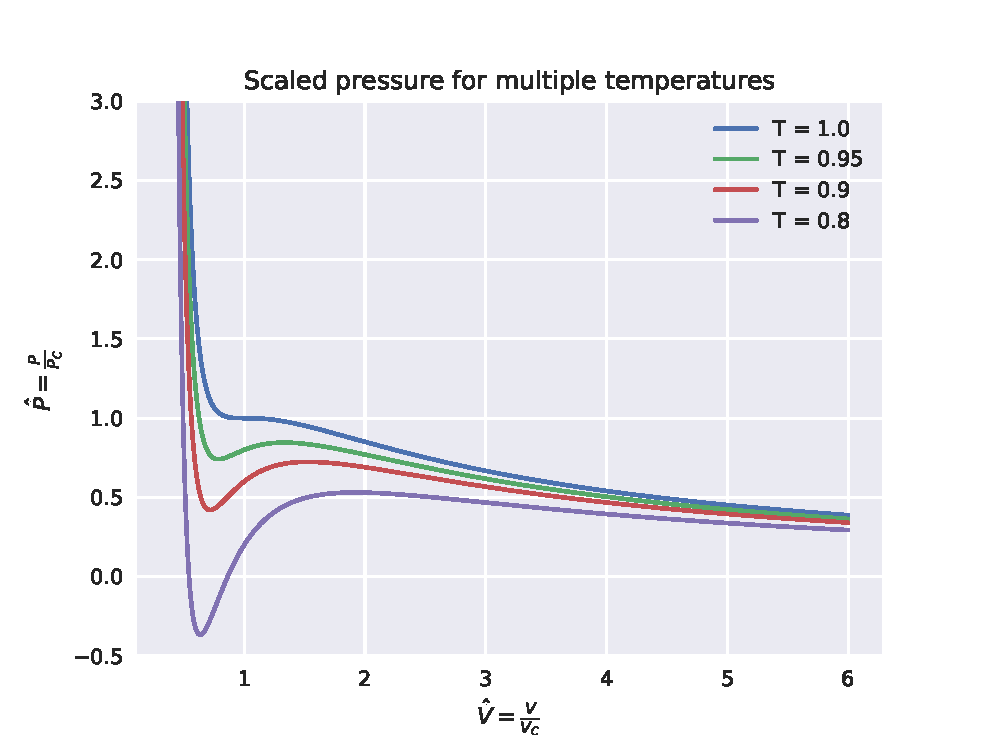
\includegraphics[width=\columnwidth]{figures/pressure_v.eps}
    \caption{Pressure vs volume}
    \label{fig:pressure}
  \end{figure}

  % Task D
  \item For the scaled quantities we have $\hat{\rho} = \frac{1}{\hat{V}}$.
  Inserting this in equation ~\ref{eq:scaledpressure} yields
  \begin{align}
    \hat{P} = \frac{8\hat{\rho}\hat{T}}{(3 - \hat{\rho})} - 3\hat{\rho}^2
  \end{align}
  which is what we wanted to show.

  %Task E
  \item See figure ~\ref{fig:pressure_density}.
  \begin{figure}[H]
    \centering
    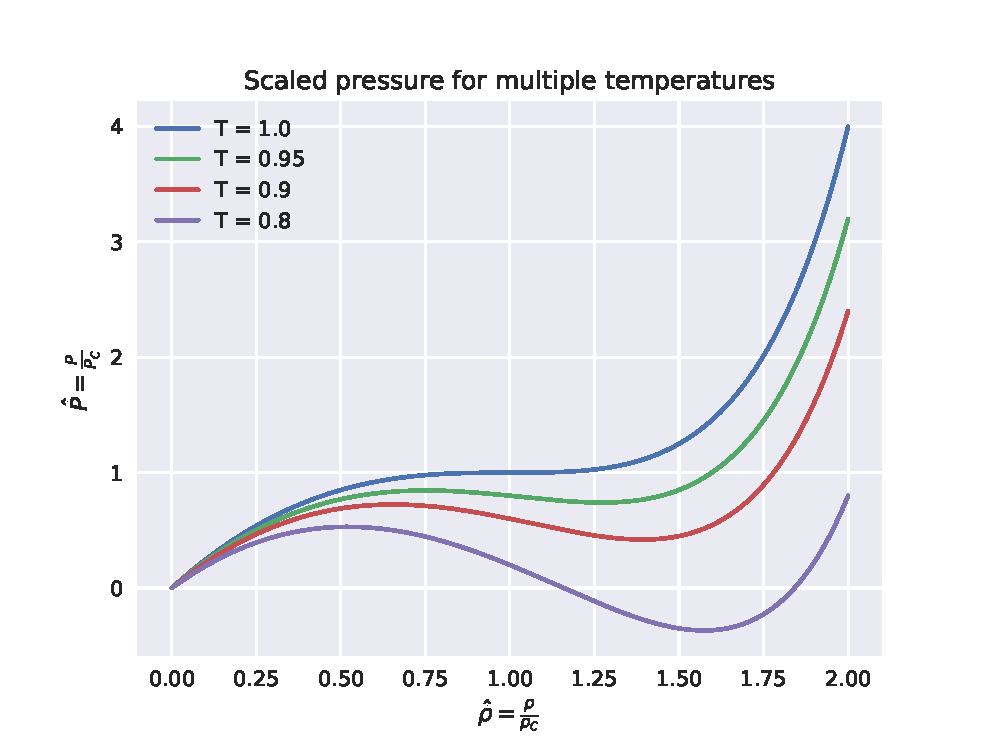
\includegraphics[width=\columnwidth]{figures/pressure_d.eps}
    \caption{Pressure vs density}
    \label{fig:pressure_density}
  \end{figure}

  % Task F
  \item Based on your plot, for what temperature does the density become
  non-unique function of the pressure?

  % Task G
  \item sumthin sumthing
\end{enumerate}

\end{document}
